\documentclass[12pt,letterpaper,final]{article}

\usepackage{Sweave}
\usepackage{graphicx}
\usepackage{natbib}
%\usepackage{hyperref}
\usepackage{caption}
\usepackage{rotating}
\usepackage{verbatim}
\usepackage{textcomp}
\usepackage[hyphens]{url}
\usepackage{latexsym}
\usepackage{wasysym}

\setlength{\oddsidemargin}{0in}
\setlength{\textwidth}{6.15in}
%\setlength{\topmargin}{0.5in}
\setlength{\textheight}{22cm}
\setlength{\headheight}{0in}
\setlength{\headsep}{0in}
\setlength{\parskip}{5pt plus 2pt minus 3pt}

\def\thefootnote{\fnsymbol{footnote}}
\setcounter{footnote}{1}

\renewcommand{\baselinestretch}{1.2}
\renewcommand{\labelenumi}{(\roman{enumi})}

\renewcommand{\topfraction}{1.0}
\renewcommand{\bottomfraction}{1.0}
\renewcommand{\textfraction}{0.0}
\renewcommand{\floatpagefraction}{1.0}

\newtheorem{definition}{Definition}
\newtheorem{theorem}{Theorem}
\newtheorem{lemma}[theorem]{Lemma}
\newtheorem{claim}[theorem]{Claim}
\newtheorem{fact}[theorem]{Fact}

% to get nice proofs ...
\newcommand{\qedsymb}{\mbox{ }~\hfill~{\rule{2mm}{2mm}}}
\newenvironment{proof}{\begin{trivlist}
\item[\hspace{\labelsep}{\bf\noindent Proof: }]
}{\qedsymb\end{trivlist}}


\newfont{\msymb}{cmsy10 scaled 1000}

\def\nullset{\mbox{\O}}
\def\R{{I\!\!R}}
\def\C{{I\!\!\!\!C}}
\def\N{{I\!\!N}}

\def\P{\mbox{\msymb P}}


%\parskip 0.1in
\pagenumbering{arabic}    %  Start using 1,2,... as page numbers.
\pagestyle{plain}         %  Page numbers in middle bottom of page.
%\setcounter{page}{80}  % XXXXXXXXXXXXXXXXX
%\setcounter{theorem}{5} % XXXXXXXXXXXXXXXXX
%\setcounter{definition}{10} % XXXXXXXXXXXXXXXXX

\parindent 0in


\begin{document}

\Sconcordance{concordance:hw01_bartschi.tex:hw01_bartschi.Rnw:%
1 122 1 1 2 1 0 8 1 1 2 3 0 1 2 21 1 1 3 6 0 1 2 21 1 1 8 7 0 1 2 1 0 1 %
1 1 2 3 1 1 4 6 0 1 2 17 1 1 4 3 0 2 1 1 5 7 0 1 2 21 1 1 6 9 0 1 2 37 %
1 1 4 3 0 2 1 1 2 1 1 1 2 1 0 1 4 7 0 1 2 14 1 1 2 5 0 1 2 15 1 1 2 5 0 %
1 2 18 1 1 2 5 0 1 2 24 1 1 2 1 0 6 1 1 4 7 0 1 2 13 1 1 2 1 0 1 1 4 0 %
1 2 80 1 1 2 1 0 2 1 1 3 1 0 1 13 12 0 1 9 7 0 1 14 12 0 1 11 13 0 1 2 %
75 1}


\begin{titlepage}
\vspace*{4.5cm}
\begin{center}
{\LARGE \bf Stat 5810, Section 003} \\[0.5cm]
{\LARGE \bf Statistical Visualization II} \\[0.5cm]
{\LARGE \bf Spring 2019} \\[0.5cm]
{\LARGE \bf Homework 1} \\[0.5cm]
~ \\[2cm]
{\bf ShaunMicheal Bartschi} \\[0.3cm]
{A01975136} \\[0.3cm]
{March 24, 2019} \\[0.3cm]
\end{center}

\thispagestyle{empty}
\vfill
\end{titlepage}

\begin{table}\centering
\begin{tabular*}{6.15in}{@{\extracolsep{\fill}}|llr|} \hline
Stat 5810/6910 Statistical Visualization II  & \hspace*{0.5 in} & Spring 2019 \\
 & & \\
\multicolumn{3}{|c|}{
Homework Assignment 1 (3/4/2019)} \\
 & & \\
\multicolumn{3}{|c|}{
90 Points --- Due Wednesday 3/20/2019 (via Canvas by 11:59pm)} \\
\hline
\end{tabular*}
\end{table}


\begin{enumerate}

\item {\bf Visualization of Multivariate Data} (60 Points): \\
In this question, you have to work with the {\it crabs} data set from the {\it MASS} package.
See the {\it crabs} help page for further details.

\begin{enumerate}
\item (3 Points) 
Load all required R packages to answer this question. Show your R code.
Do not just blindly trust the information on the help page! How many observations 
and how many variables are included 
in this data set overall? \\

Use something like the following to incorporate results from your R code directly
into your \LaTeX\ text:
``Apparently, there are 50 observations
and 2 variables
in the cars data set.'' \\


\underline{Answer:}
{\scriptsize
\begin{Schunk}
\begin{Sinput}
> setwd("C:/Users/Shaun/Desktop/StatVis/StatVis2/HW1")
> library(ggplot2)
> library(MASS)
> library(lattice)
> library(GGally)
> library(dplyr)
> library(PairViz)
> library(RColorBrewer)
> library(gplots)
> data(crabs)
\end{Sinput}
\end{Schunk}

There are 200 observations
and 8 variables
in the {\it crabs} data set. \\
}


\item (4 Points) 
Create a default scatterplot matrix 
of the five quantitative variables (omitting {\it sp, sex \& index})
via {\it baseR}. Do not optimize
this scatterplot matrix and do not use any colors or symbols.
Describe this scatterplot matrix. Which questions naturally come to your mind?
What would you initially anticipate as the answers to your questions?
Do not modify your answer here, even if it turns out later on that your
anticipation was not correct!
Hint: Think of which variables have been ignored in your scatterplot matrix.
Include your figure and your R code. \\


\underline{Answer:}
{\scriptsize
\begin{Schunk}
\begin{Sinput}
> pairs(crabs[,4:8],
+       main="Default Scatterplot Matrix")
\end{Sinput}
\end{Schunk}
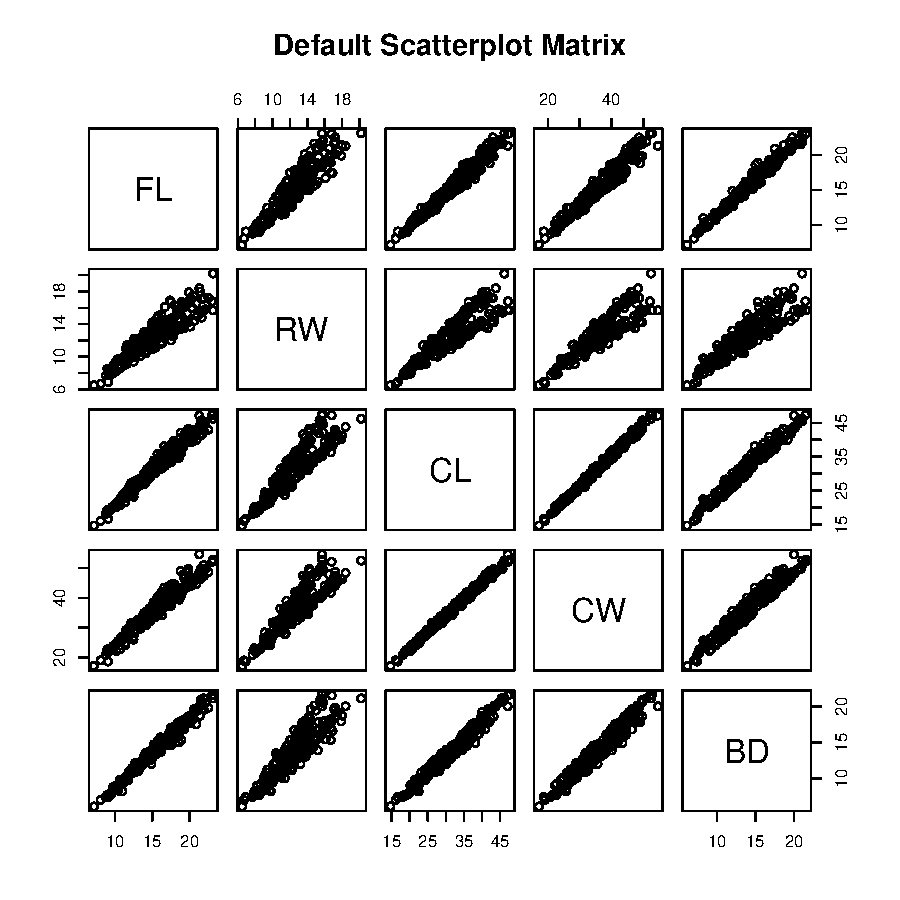
\includegraphics{hw01_bartschi-002}

There appears to be a strong linear correlation between the variables, so we might assume that this correlation might also hold between the variables {\it sp} and {\it sex}.
}


\item (5 Points) 
Redo your scatterplot matrix from part (b)
of the five quantitative variables (omitting {\it sp, sex \& index})
via {\it baseR}. Now use different colors and symbols.
Recall that ``B'' represents blue crabs and ``O'' represents orange crabs,
so use these two colors.
Use ``o'' to represent male crabs and ``+'' to represent female crabs.
This is a perfect opportunity to make use of ``ifelse'' expressions
in your R code!
Also reduce the symbol size ({\it cex}) to 0.5.
Describe this scatterplot matrix. Does this answer your previous questions from part (b)?
Was your anticipation correct?
Include your figure and your R code. \\


\underline{Answer:}
{\scriptsize
\begin{Schunk}
\begin{Sinput}
> # data(state)
> # tristate <- as.data.frame(state.x77[, c(3, 6, 5)])
> # illiteracy <- tristate[, 1]
> # grad <- tristate[, 2]
> # pairs(tristate, col = unclass(state.region))
> 
> cols <- character(nrow(crabs))
> #cols[] <- "black"
> cols[crabs$sp == "B"] <- "blue"
> cols[crabs$sp == "O"] <- "orange"
> shapes <- character(nrow(crabs))
> shapes[] <- 0
> shapes[crabs$sex == "F"] <- '1'
> shapes[crabs$sex == "M"] <- '3'
> pairs(crabs[,4:8],
+      main="Improved Scatterplot Matrix",
+      col = unclass(cols), pch = c(1,3)[as.numeric(crabs$sex)], cex = 0.5)
\end{Sinput}
\end{Schunk}
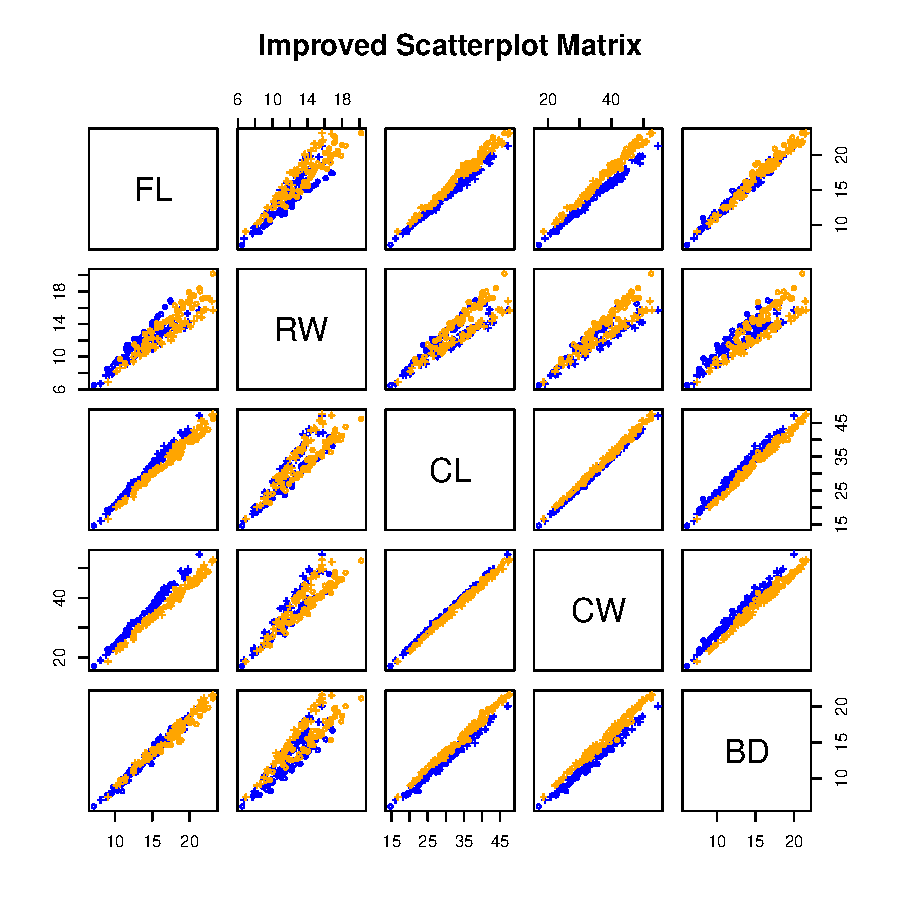
\includegraphics{hw01_bartschi-003}

It would seem that my anticipation was correct, and that there is some correlation between gender and color as well.
}


\item (4 Points) 
Redo your scatterplot matrix from part (c)
of the five quantitative variables (omitting {\it sp, sex \& index})
via {\it ggpairs}.
Use the same colors and symbols as in part (c).
For everything else,
use the default settings and show the four densities on the diagonal
and the correlations in the upper triangular matrix.
Include your figure and your R code. \\


\underline{Answer:}
{\scriptsize
\begin{Schunk}
\begin{Sinput}
> ggplot <- function(...) ggplot2::ggplot(...) + 
+   scale_color_manual(values = c("blue","orange")) +
+   scale_fill_manual(values = c("blue","orange"))
> unlockBinding("ggplot",parent.env(asNamespace("GGally")))
> assign("ggplot",ggplot,parent.env(asNamespace("GGally")))
> ggpairs(crabs, columns = 4:8,
+         title = "GGplot Scatterplot Matrix",
+         aes(color = cols, shape = shapes),
+         upper = list(continuous = wrap("cor", size = 2.25)))
\end{Sinput}
\end{Schunk}
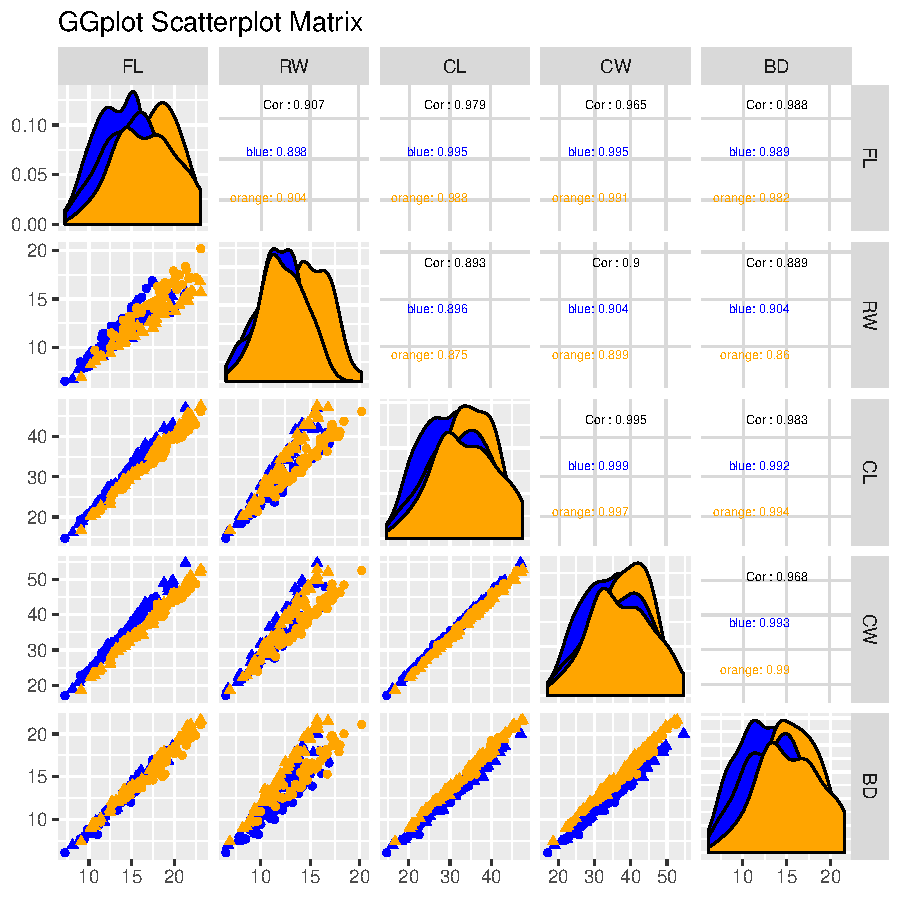
\includegraphics{hw01_bartschi-004}


}


\item (5 Points) 
Redo your scatterplot matrix from part (d)
of the five quantitative variables including {\it sp \& sex} 
(but still omitting {\it index})
via {\it ggpairs}. 
Place {\it sp \& sex} after the five quantitative variables so that
the histograms and box plots appear on the bottom and on the right.
Use the same colors and symbols as in part (d).
Choose 10 bins for all histograms.
For everything else,
use the default settings and show the four densities on the diagonal
and the correlations in the upper triangular matrix.
Include your figure and your R code. \\


\underline{Answer:}
{\scriptsize
\begin{Schunk}
\begin{Sinput}
> ggpairs(crabs, columns = c(4:8,1:2), 
+         title = "Expanded GGplot Scatterplot Matrix",
+         aes(color = cols, shape = shapes),
+         lower = list(combo = wrap("facethist", bins = 10)),
+         upper = list(continuous = wrap("cor", size = 1.5)))
\end{Sinput}
\end{Schunk}
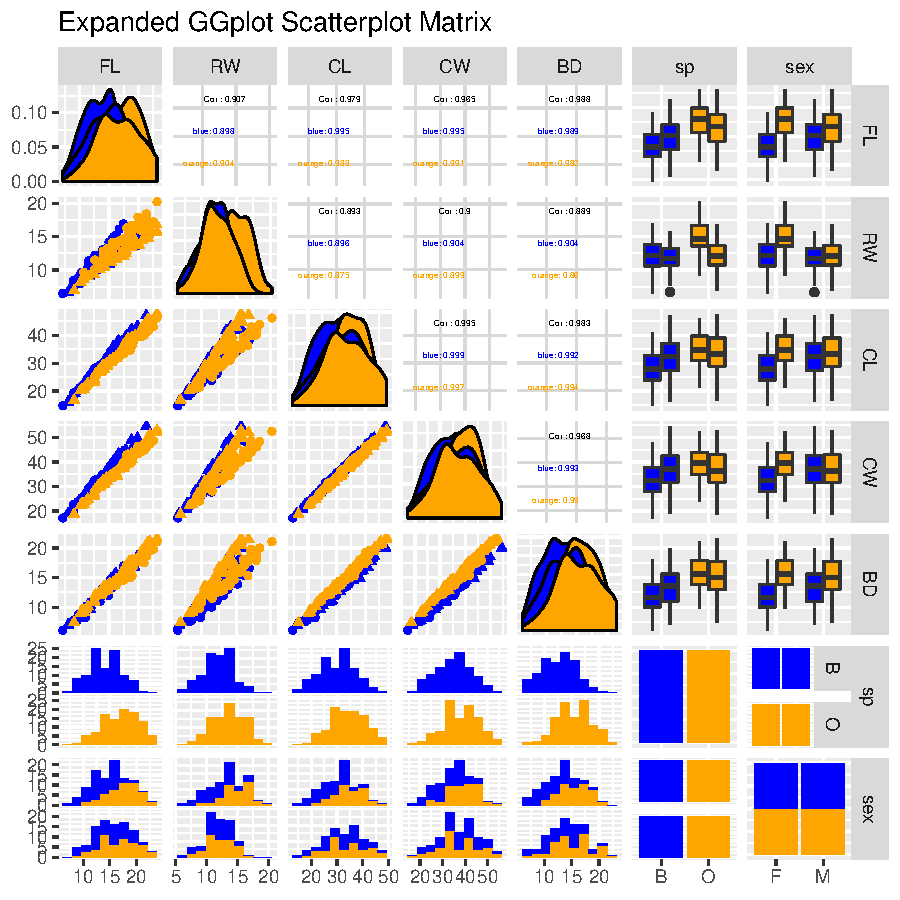
\includegraphics{hw01_bartschi-005}
}


\item (6 Points) 
Frankly, I have a problem with the interpretation of the
(extended) scatterplot matrix from part (e). 
Can you easily identify which boxplot and
histogram belongs to which species or which sex?
Therefore, do the following: Add an ``interaction variable'' of {\it sp.sex}
to the crabs data set. Recall how we did this for ``SexClassSurvived''
for the Titanic data set. {\bf Reorder your factor levels as
B.M, B.F, O.M, and O.F. Do not leave the factor levels in the order that was produced by R.}
We have done such reorderings of factor levels in {\it Statistical Visualization I}.

Redo your scatterplot matrix from part (e), but now with {\it sp.sex} as the
only categorical variable. Use a diverging 4--class {\it RdYlBu} color scheme from the
{\it RColorBrewer} R package where 
``blue'' represents blue crabs and ``red'' represents orange crabs.
Use the two darker (outside) colors for the male crabs and the 
two fainter (inside) colors for the female crabs. Warning: Make sure
that you correctly map these colors to the species and sex.
If you are not certain, compare with your scatterplot matrix from {\it baseR}.

As before, choose 10 bins for all histograms.
For everything else,
use the default settings and show the four densities on the diagonal
and the correlations in the upper triangular matrix.
Reduce alpha to 0.5 address the overplotting problem.
Likely, your font size will be too large for the values of the correlations.
Also check and adjust the font sizes on the axes if necessary.
Recall that this has to look good in your final pdf version and
not in the Plots window in RStudio. If necessary,
google for a solution how to adjust the font sizes in {\it ggpairs}.
Include your figure and your R code. \\


\underline{Answer:}
{\scriptsize
\begin{Schunk}
\begin{Sinput}
> ggplot <- function(...) ggplot2::ggplot(...) +
+   scale_color_manual(values = rev(brewer.pal(5,"RdYlBu"))) +
+   scale_fill_manual(values = rev(brewer.pal(5,"RdYlBu")))
> unlockBinding("ggplot",parent.env(asNamespace("GGally")))
> assign("ggplot",ggplot,parent.env(asNamespace("GGally")))
> crabs.ordered <- crabs
> crabs.ordered$interaction <- with(crabs, interaction(sp, sex))
> crabs.ordered$interaction <- factor(crabs.ordered$interaction,
+                                     levels = c("B.M", "B.F", "O.M", "O.F"))
> ggpairs(crabs.ordered, columns = 4:9, 
+         title = "Improved GGplot Scatterplot Matrix",
+         aes(color = crabs.ordered$interaction),
+         lower = list(combo = wrap("facethist", bins = 10)))
\end{Sinput}
\end{Schunk}
\includegraphics{hw01_bartschi-006}
}


\item (4 Points) 
Create a default parallel coordinates plot (PCP) 
of the five quantitative variables (omitting {\it sp, sex \& index})
via {\it baseR}. Do not optimize
this PCP and do not use any colors.
Describe this PCP. Are there any variables that allow to separate 
one of the species or sexes?
Include your figure and your R code. \\


\underline{Answer:}
{\scriptsize
\begin{Schunk}
\begin{Sinput}
> parcoord(crabs.ordered[,4:8], main = "Parallel Coordinate Plot")
\end{Sinput}
\end{Schunk}
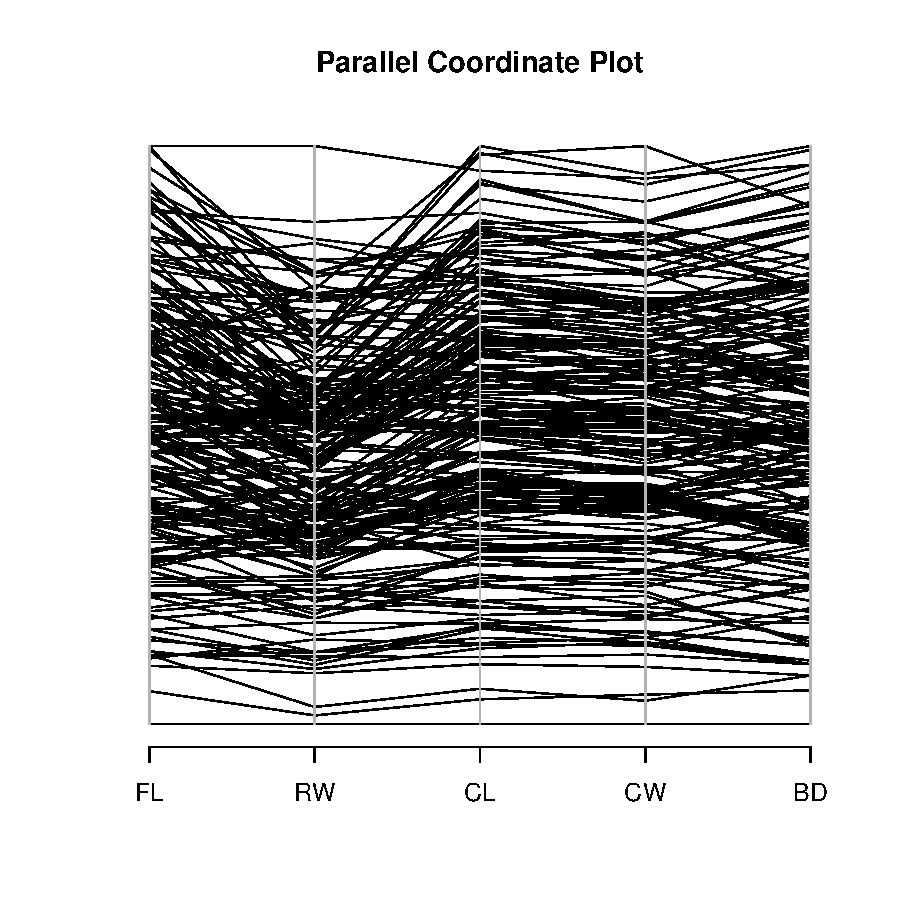
\includegraphics{hw01_bartschi-007}

It would appear that there is at least two patterned groups that would be a valid show of gender's influence on the other factors.  The one that sticks out most prominently is the variable {\it RW}.
}


\item (5 Points) 
Redo your PCP from part (g)
of the five quantitative variables (omitting {\it sp, sex \& index})
via {\it baseR}. Now use the same colors as in part (f). 
Are there any variables that allow to partially separate 
one of the species or sexes?
Include your figure and your R code. \\


\underline{Answer:}
{\scriptsize
\begin{Schunk}
\begin{Sinput}
> parcoord(crabs.ordered[,4:8], col = rev(brewer.pal(5,"RdYlBu")[unclass(crabs.ordered$interaction)]))
\end{Sinput}
\end{Schunk}
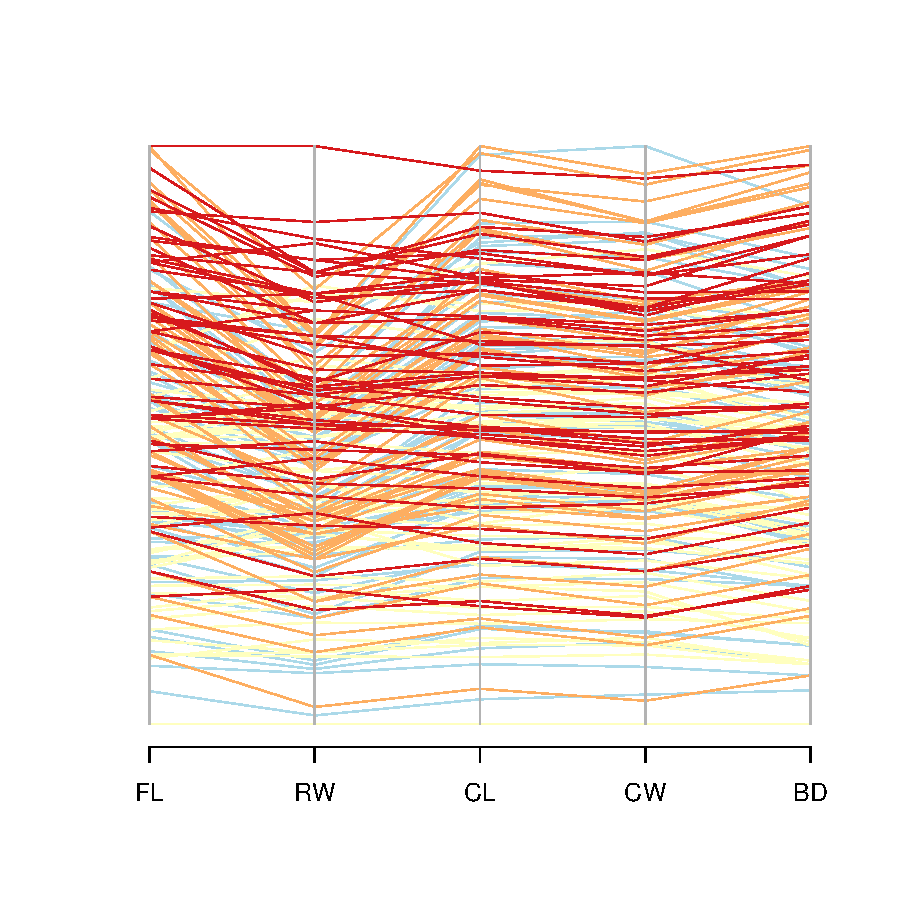
\includegraphics{hw01_bartschi-008}
}




\item (5 Points) 
Redo your PCP from part (h)
of the five quantitative variables (omitting {\it sp, sex \& index})
via the {\it ggparcoord} function from the {\it GGally} R package. 
Use the same colors as in part (f). 
Use a 0--1--scale for all parallel axes.
Hint: The legend of this graph should reveal whether you correctly 
use the colors as specified in part (f). If something goes wrong here,
likely you use the colors incorrectly in some of your previous parts as well.
Include your figure and your R code. \\


\underline{Answer:}
{\scriptsize
\begin{Schunk}
\begin{Sinput}
> ggparcoord(crabs.ordered, columns = 4:8, groupColumn = 9, scale = "uniminmax")
\end{Sinput}
\end{Schunk}
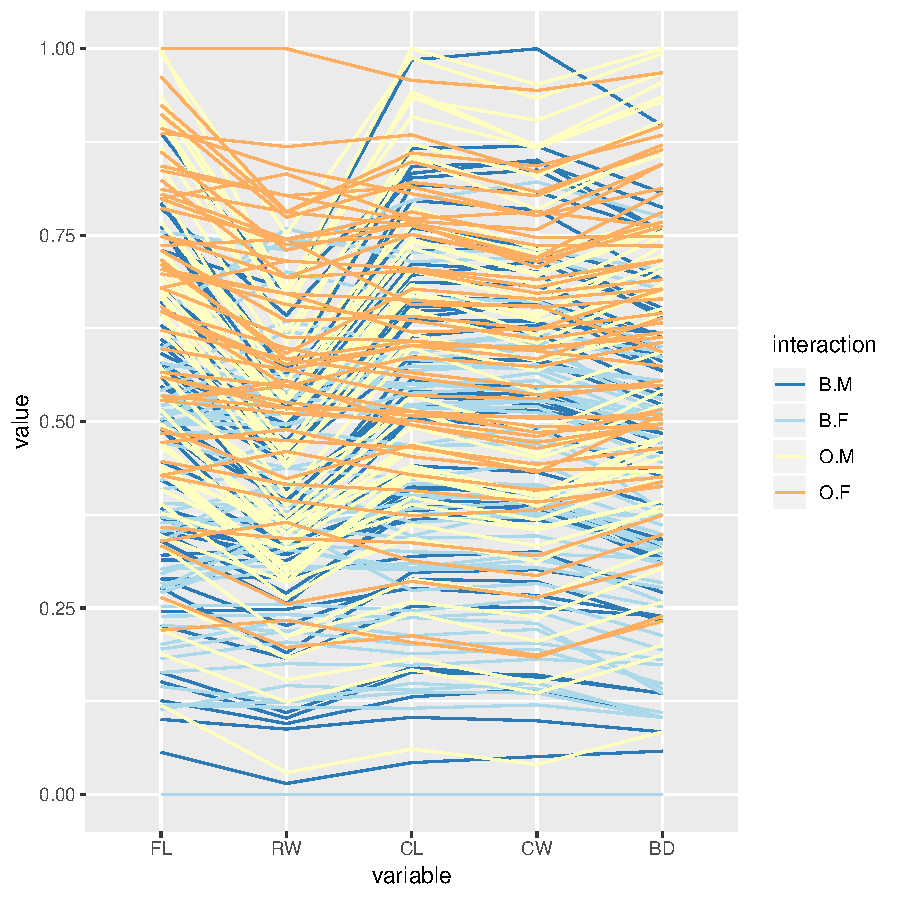
\includegraphics{hw01_bartschi-009}
}


\item (6 Points) 
Let's try something: First install the {\it BiocManager} R package from CRAN.
Then install the {\it graph} R package from Bioconductor as follows:
\begin{verbatim}
BiocManager::install("graph", version = "3.8")
\end{verbatim}
Finally install the {\it PairViz} R package from CRAN.
Read the PCP vignette at 
\url{https://cran.r-project.org/web/packages/PairViz/vignettes/pcp.html}.

Adapt the example code to create a 
``Weighted Eulerian with Correlation Guide,'' placing the bars for the
correlations below the PCP. 
Do not color--code the lines in the PCP. Describe and
interpret this version of the PCP (recall the made--up examples from class).
It will also be helpful to revisit the
correlations in the scatterplot matrix in part (f).
Include your figure and your R code. \\


\underline{Answer:}
{\scriptsize
\begin{Schunk}
\begin{Sinput}
> data <- crabs[4:8]
> corw <- as.dist(cor(data))
> o <- eulerian(-corw)
> par(cex.axis=.7)
> corw <- dist2edge(corw)
> edgew <- cbind(corw*(corw>0), corw*(corw<0))
> par(cex.axis=.7)
> guided_pcp(data,edgew, path=o,pcp.col="grey50" ,lwd=2,
+          main="Weighted eulerian with correlation guide",
+          bar.col = c("lightpink1","lightcyan1"),
+          bar.ylim=c(-1,1),bar.axes=TRUE)
\end{Sinput}
\end{Schunk}
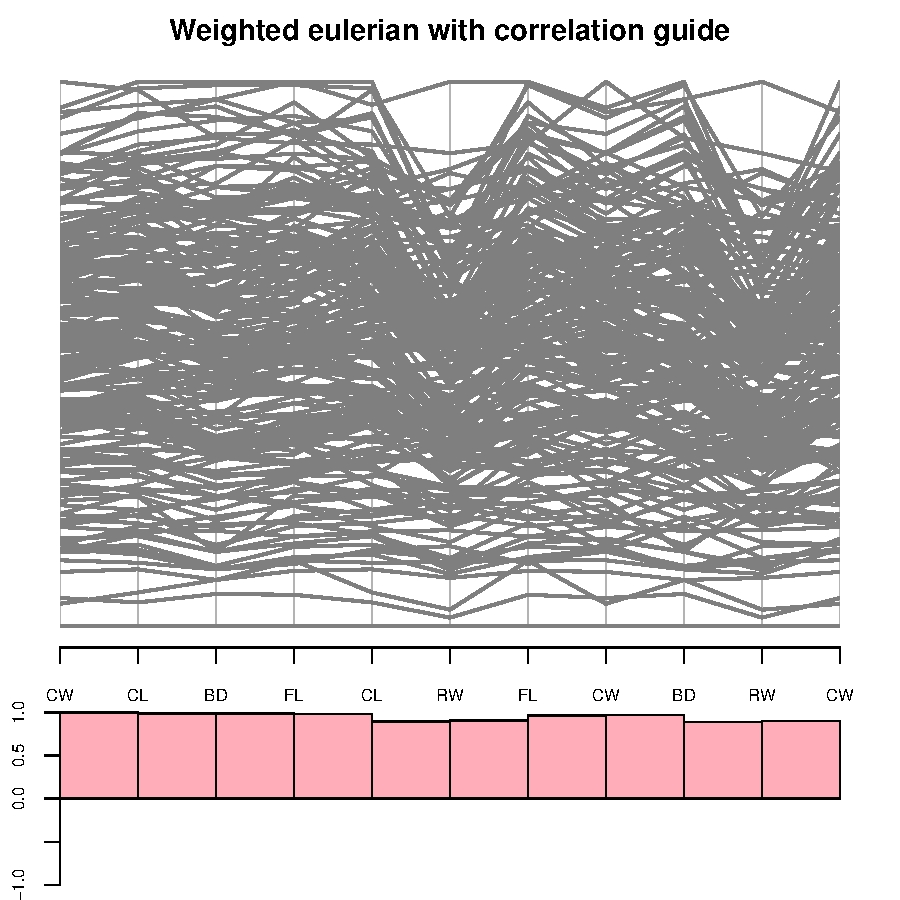
\includegraphics{hw01_bartschi-010}
}


\item (5 Points) 
Create a heatmap
of the five quantitative variables (omitting {\it sp, sex \& index})
via the {\it heatmap.2} function from the {\it gplots} R package.
Make sure to scale your variables!
What can we learn from this heatmap (if anything at all)?
Include your figure and your R code. \\


\underline{Answer:}
{\scriptsize
\begin{Schunk}
\begin{Sinput}
> crabs48 <- as.matrix(crabs[4:8])
> heatmap.2(scale(crabs48))
\end{Sinput}
\end{Schunk}
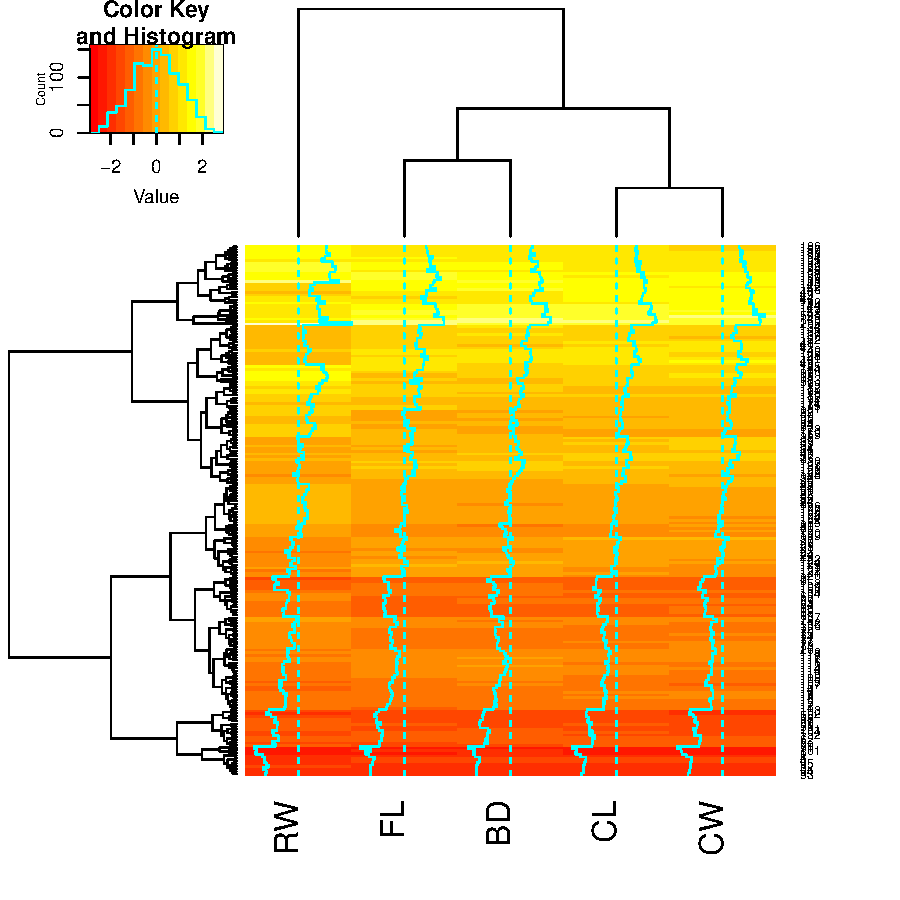
\includegraphics{hw01_bartschi-011}

It appears as though there does exist strong correlation between the factor levels moving from smallest value to highest value.
}


\item (8 Points) 
Start with a basic description of the data set and its variables. Then provide a detailed interpretation of your graphical results. Point out differences and similarities for the two species and the two sexes.  Also comment  on  similarities  of  the  variables. Do this for the univariate graphical summaries of the five quantitative variables, the pairwise scatterplots  of these variables, the PCPs, and the heatmap. Compare and combine results obtained from the various graphs.  Ideally, different graphs should result in similar interpretations, but, if necessary, point out when different graphs result in contradictory interpretations.  Be specific and refer back to specific question parts and do not just say "the PCP or the scatterplot matrix shows shows $\ldots$''.\\
This summary should be at least 1 page in length. \\


\underline{Answer:}
{\scriptsize
I believe that each of these plots convey the fundamental correlation between each of the factor levels, including {\it species} and {\it sex}.  I believe that the Matrix plots from parts (b)-(f) hammer home this point, with particular emphasis on part (f) which included information on distributions, correlation, and box plots for
}
\end{enumerate}


\newpage


\item {\bf From Tables to Graphs} (30 Points): \\
You have to 
find a suitable table and translate this table into a graph.
This must be a ``multivariate'' (non--trivial) table with several variables,
possibly with different estimates, confidence intervals, etc. 
A table that could just be translated into several columns of dotplots is not acceptable. \\

%\underline{Comment:} \\
%{\bf Answers will differ, depending on the selected table.} \\


\begin{enumerate}
\item (5 Points)
Present your proposed table to me after class, during office hours, or
via e--mail by {\bf Sunday 3/10/2019, 11:59pm}
to get my approval before you start translating it into a graph.

The table should have been published in the last four years (2016 to 2019).
It can originate from a journal or conference proceedings article, textbook, or from the Web.
If you can find a suitable table related to your MS or PhD research
(or from your main adviser), that would be perfect.
Include the reference where you located the table.\\

Table is included below.  Primary report was generated by Lieutenant Mikelshan Bartschi on March 10, 2019 citing the number of 'Calls to Service' performed by the Cache County Sheriff's Office in the previous year by weekday and hour.

\item (15 Points)
You should review the section titled {\it From Tables to Plots} 
in our lecture notes before you start with your conversion.
Also, take a closer look at the references cited in that section and under {\it Further Reading}.
Examples 1 and 2 from that section might provide you with useful R commands.
The {\tt barley} example from {\it Statistical Visualization I}
may also provide you with some useful design suggestions and R commands.

Moreover, take a look at the examples in the section titled {\it Linked Micromap Plots}.
Even if your table is not related to any geographic data, the other
components from linked micromap plots may still be useful for your conversion.
For example, see how we have displayed confidence bounds (or minima and maxima),
population means (or medians), annual changes, and even time series in micromaps.
The same principles may be suitable for your conversion.

In addition to the graph types mentioned above, some tables may be
translated into parallel coordinate plots, time series plots, or 
graphs that are based on the small multiples principle.
Ultimately, it is your decision which design to choose for your graph.

One suggestion: Before you code your graph in R, manually design the layout 
of your graph on paper. 
Recall from {\it Statistical Visualization I}
that even a tiny data set allows us to draw many different graphs. 
It is likely that you need to consider several possible designs for your graph
first before you come up with a design that best highlights the information
from the table. 

Now go ahead and translate your table into a graph!
Include the original table, the final
version of your graph, and the R code that was used to create your graph
as an answer to this question.\\

\underline{Original Table:}\\
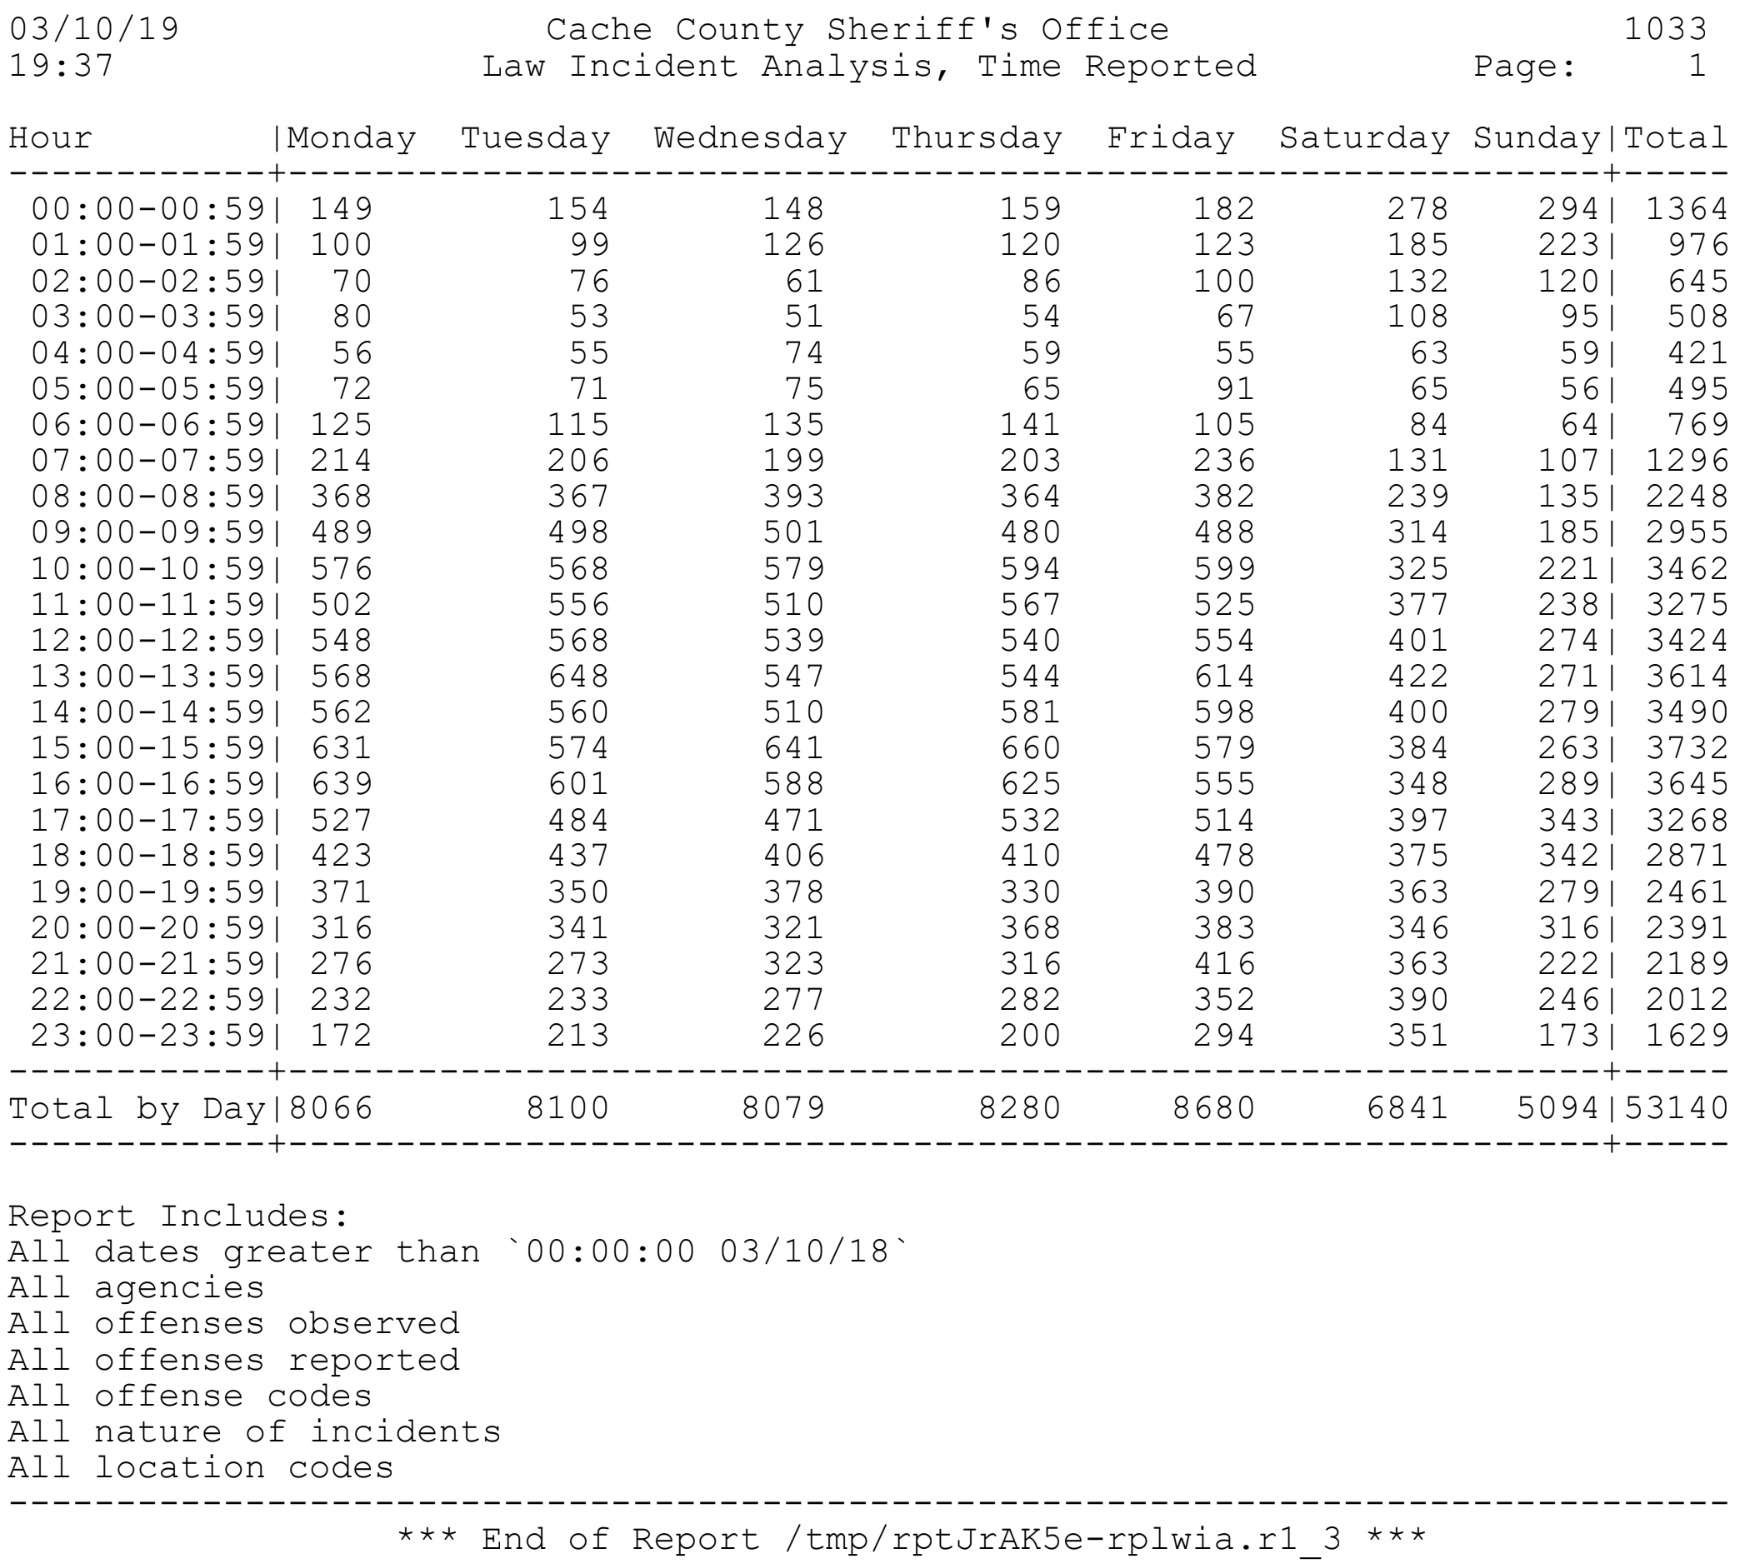
\includegraphics[width = 5.5 in]{table_allCalls.PNG}\\
\underline{Code and Final graphical Visualization:}\\
\begin{Schunk}
\begin{Sinput}
> ggplot <- function(...) ggplot2::ggplot(...)
> unlockBinding("ggplot", parent.env(asNamespace("GGally")))
> assign("ggplot", ggplot, parent.env(asNamespace("GGally")))
> temp <- read.table("allCalls.csv", header=TRUE,
+                         sep=",", stringsAsFactors = FALSE)
> all.Calls <- data.frame(Hour = rep(temp$Hour,7),
+                    Day = c(rep("Monday",24), 
+                            rep("Tuesday",24), 
+                            rep("Wednesday",24), 
+                            rep("Thursday",24), 
+                            rep("Friday",24), 
+                            rep("Saturday",24), 
+                            rep("Sunday",24)
+                            ),
+                    Calls = c(temp$Monday, temp$Tuesday, 
+                             temp$Wednesday, temp$Thursday, 
+                             temp$Friday, temp$Saturday, 
+                             temp$Sunday))
> all.Calls$Day <- factor(all.Calls$Day,
+                         levels = c("Monday", 
+                                    "Tuesday", 
+                                    "Wednesday", 
+                                    "Thursday", 
+                                    "Friday", 
+                                    "Saturday", 
+                                    "Sunday"))
> all.Calls$Hour <- factor(all.Calls$Hour,
+                          levels = c("04:00-04:59","05:00-05:59",
+                                     "06:00-06:59","07:00-07:59",
+                                     "08:00-08:59","09:00-09:59",
+                                     "10:00-10:59","11:00-11:59",
+                                     "12:00-12:59","13:00-13:59",
+                                     "14:00-14:59","15:00-15:59",
+                                     "16:00-16:59","17:00-17:59",
+                                     "18:00-18:59","19:00-19:59",
+                                     "20:00-20:59","21:00-21:59",
+                                     "22:00-22:59","23:00-23:59",
+                                     "00:00-00:59","01:00-01:59",
+                                     "02:00-02:59","03:00-03:59"))
> # basic line plot for personal reference
> # ggplot(data = all.Calls, aes(x=Hour,y=Calls,group=Day)) + 
> #   geom_line(aes(color=Day)) + 
> #   theme(axis.text.x = element_text(angle = 45, hjust = 1)) + 
> #   scale_color_brewer(palette = "Spectral")
> 
> ggparcoord(all.Calls, columns = c(1,3), groupColumn = 2, 
+            scale = "uniminmax", 
+            title = "Annual Calls to Service Breakdown 
+            by Hour and Day")
\end{Sinput}
\end{Schunk}
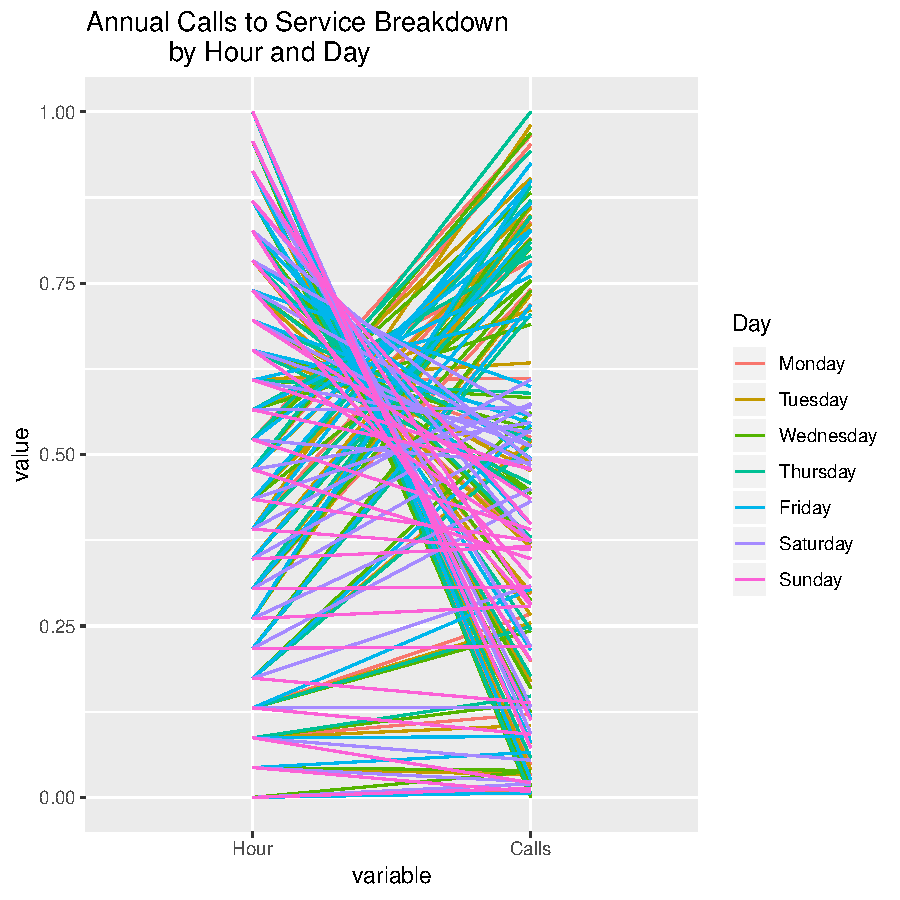
\includegraphics{hw01_bartschi-012}

\item (10 Points)
In addition to translating the table into a graph, 
you have to explain and motivate your resulting graph!
Why did you choose that particular graph design? What sorting
did you use for the rows and columns of the original table?
How (and why) did you combine data from the table, e.g., means
and standard deviations from the table into means and confidence intervals
in your graph? How (and why) did you choose specific colors
and glyphs in your graph, etc.?

Also emphasize what are the most important features that can be seen
in your graph. Keep in mind that the general audience may have never
seen such a graph type before. So, you may have to explain some
of the basic design features of your graph.
{\scriptsize
\underline{Motivation:}\\
I chose this particular graph design because I believe that it quickly allows an individual to see that the number of calls is much higher in the middle of the day than in the morning or night.  As is, this graph would stilll need to be explained to the law enforcement audience, as they would need to be told how to interpret the hours (since I modified the order to start at 4am and end at 3 am).  This could be clarified by better labeling, although it could very well croud the graph with text.  Ultimately, the intent of this graph is to make it quickly apparent that there are trends between the hour of the day and the calls, and upon closer inspection, also the day of the week that it occured.  I would likely pair this plot with the more basic line plot that I created as well to increase informational awareness.
}

\end{enumerate}

\end{enumerate}


\newpage


\noindent{\Large \bf General Instructions}~\\


\begin{enumerate}
\item Create a single pdf document, using R Markdown, Sweave, or knitr.
When you take this course at the 6000--level, you have to use \LaTeX\ in
combination with Sweave or knitr.
You only have to submit this one document.

\item Include a title page that contains your name, your A--number, the number of
the assignment, the submission date, and any other relevant information.

\item Start your answers to each main question on a new page (continuing with the next
part of a question on the same page is fine). 
Clearly label each question and question part.

\item Show your R code for each question part!

\item Before you submit your homework, check that you
follow all recommendations from Google's R Style Guide
(see \url{https://google.github.io/styleguide/Rguide.xml}). 
Moreover, make sure that your R code is consistent, i.e., that you use the same
type of assignments and the same type of quotes throughout your entire homework.

\item Give credit to external sources, such as stackoverflow or help pages. Be specific
and include the full URL where you found the help (or from which help page you got 
the information). Consider R code from such sources as ``legacy code or third--party code'' 
that does not have to be adjusted to Google's R Style (even though it would be nice,
in particular if you only used a brief code segment).

\item {\bf Not following the general instructions outlined above will result in point deductions!}

\item For general questions related to this homework, please
use the corresponding discussion board in Canvas! I will try to
reply as quickly as possible. Moreover, if one of you knows
an answer, please post it. It is fine to refer to web pages
and R commands, but do not provide the exact R command with all required arguments
or which of the suggestions from a stackoverflow web page eventually worked for you! 
This will be the task for each individual student!

\item Submit your single pdf file via Canvas by the submission deadline.
Late submissions will result in point deductions as outlined on the syllabus.

\end{enumerate}


\end{document}

